% ============================================================
\section{Spherical Harmonics}
\label{sec:sh}

Spherical harmonics are the Fourier series for the sphere, and are an important tool for solving numerical problems involving the spherical domain. They are often derived as eigensolutions to the surface Laplacian, which is the analog to developing the Fourier series as eigensolutions of the operator $(d/dx)^2$ on a finite line with the boundary conditions that $y$ and $dy/dx$ match at the two ends (see Riley et al.~\cite{Riley2006}). The result of this derivation are complex-valued functions $\SHBC$, which are defined as:
\begin{align}
\label{eq:sh_definition}
\SHBC^{l,m}(\theta, \phi)=
\begin{cases}
C^{l,m}e^{im\phi}P^{l,m}\left(\operatorname{cos}\theta\right), & \text{for $m\ge0$}\\
\left(-1\right)^m\overline{\SHBC^{l\left|m\right|}}(\theta, \phi), & \text{for $m<0$}
\end{cases}
\quad ,
\end{align}
where $P^{l,m}$ are the associated Legendre polynomials. While those can be defined in many different ways, the most numerically robust way to evaluate them is by using the following set of recurrence relations (Press et al.~\cite{Press07}):
\begin{align}
P^{0,0}\left(\operatorname{cos}\theta\right) &=
1
\  ,
\nonumber
\\
P^{m,m}\left(\operatorname{cos}\theta\right) &=
\left(2m-1\right)!!\left(1-\operatorname{cos}^2\theta\right)^\frac{m}{2}
\  ,
\nonumber
\\
P^{m+1,m}\left(\operatorname{cos}\theta\right) &=
\operatorname{cos}\theta\left(2m+1\right)P^{m,m}\left(\operatorname{cos}\theta\right)
\ 
\nonumber
\\
P^{l,m}\left(\operatorname{cos}\theta\right) &=
\frac{\operatorname{cos}\theta\left(2l-1\right)}{l-m}
P^{l-1,m}\left(\operatorname{cos}\theta\right)
-
\frac{l+m-1}{l-m}
P^{l-2,m}\left(\operatorname{cos}\theta\right)
\  .
\label{eq:sh_Plm}
\end{align}
The factor $C^{l,m}$ in equation~\ref{eq:sh_definition} is defined as
\begin{align}
\label{eq:sh_definition_C}
C^{l,m}=(-1)^m\sqrt{\frac{2l+1}{4\pi}\frac{(l-m)!}{(l+m)!}}
\end{align}
Since spherical harmonics are used in many different fields, their definition can vary and one has to be careful, when comparing them across literature. This concerns the $(-1)^m$ factor in particular, which is called the Condon-Shortley phase. Sometimes, this factor is part of the definition of the associated Legendre polynomial $P^{l,m}$ and therefore does not appear in $C^{l,m}$. More importantly, the definition of $C^{l,m}$ depends on how the spherical harmonics are expected to be normalized.
\newline
\begin{figure}[h]
\centering
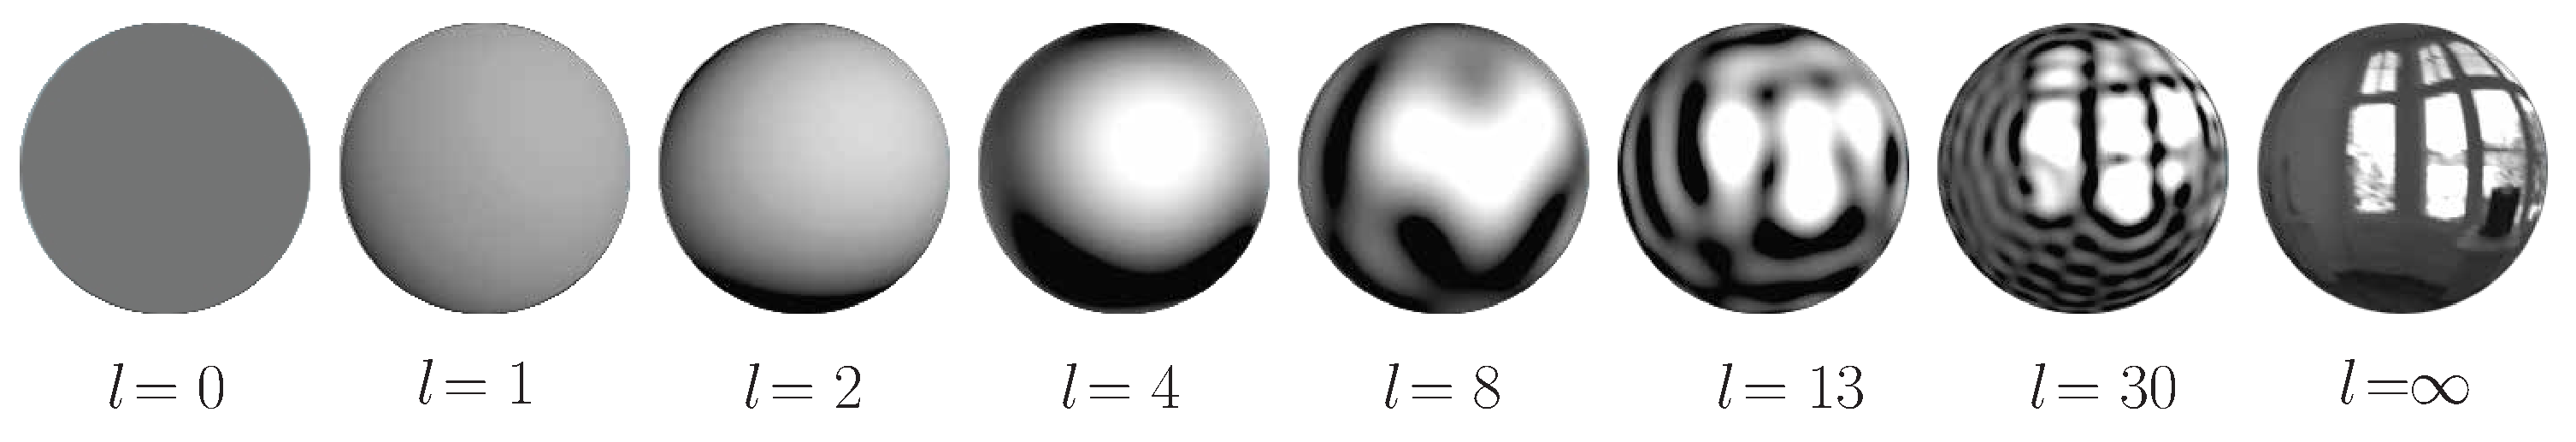
\includegraphics[width=\columnwidth]{04_pn_method/figures/fig_sph_frequencies.pdf}
\caption{Approximating a spherical function using spherical harmonics with increasing truncation order (from left to right). Like with the Fourier-transform, higher truncation order allows capturing higher frequencies.}
\label{fig:sh_vis}
\end{figure}


%\begin{figure}[h]
%\centering
%\begin{subfigure}{0.31\columnwidth}
%%\includegraphics[width=\columnwidth]{images/checkerboard2d_p1_neumann_staggered_starmap.png}
%%spherical harmonics basis function hierarchy in 2d
%\missingfigure{see comment}
%\caption{TODO}
%\label{fig:sh_vis_1}
%\end{subfigure}
%\hspace{0.01\columnwidth}
%\begin{subfigure}{0.31\columnwidth}
%%\includegraphics[width=\columnwidth]{images/checkerboard2d_p1_neumann_staggered.png}
%%some environment map and truncated reconstruction in 2d
%\missingfigure{see comment}
%\caption{TODO}
%\label{fig:sh_vis_2}
%\end{subfigure}
%\hspace{0.01\columnwidth}
%\begin{subfigure}{0.31\columnwidth}
%%\includegraphics[width=\columnwidth]{images/checkerboard2d_p1_neumann_staggered.png}
%%the hierarchy for the reconstruction with weights
%\missingfigure{see comment}
%\caption{TODO}
%\label{fig:sh_vis_3}
%\end{subfigure}%
%\caption{TODO}
%\label{fig:sh_vis}
%\end{figure}

\subsubsection*{Normalization and Orthogonality}

The coefficient $C^{l,m}$ has been defined as such that the spherical harmonics function $\SHBC$ scales to the unit norm
\begin{align}
\label{eq:sh_normalization}
\norm{\SHBC^{l,m}} = \sqrt{\left<\SHBC^{l,m}, \SHBC^{l,m}\right>} = 1
\ .
\end{align}
Other spherical harmonics definitions use a different constant (e.g. $4\pi$) and therefore arrive at different $C^{l,m}$. Since the spherical harmonics functions $\SHBC$ are complex-valued functions on the unit sphere, they are elements of the Hilbert space, for which the inner product is defined as:
\begin{align}
\label{eq:sh_inner_product}
\left<f,g\right> = \int_\Omega f\left(\vec{\omega}\right)\overline{g}\left(\vec{\omega}\right)\ud\vec{\omega}
\end{align}
with $\overline{g}$ being defined as the complex conjugate of $g$ (Folland~\cite{Folland92}).

The spherical harmonics functions form a orthogonal family and thus result in:
\begin{align}
\left<\SHBC^{l_1, m_1},\SHBC^{l_2, m_2}\right>
=
0
\ ,\quad\text{ for } l_1 \ne l_2 \text{ and } m_1 \ne m_2
\end{align}
The properties of normalization (equation~\ref{eq:sh_normalization}) and orthogonality (equation~\ref{eq:sh_orthogonality}) give
\begin{align}
\label{eq:sh_orthogonality}
\left<\SHBC^{l_1, m_1},\SHBC^{l_2, m_2}\right>=
\int_{\Omega} \SHBC^{l_1m_1}\left(\vec{\omega}\right) \overline{\SHBC^{l_2m_2}}\left(\vec{\omega}\right) \mathbf{d}\vec{\omega} = \delta_{l_1m_1}\delta_{l_2m_2}
\ .
\end{align}

\subsubsection*{Projection and Reconstruction}

Because the spherical harmonics are orthonormal, a spherical functional $f\left(\vec{\omega}\right)$ can be projected into scalar spherical harmonics basis function coefficients $f^{l,m}$, using the inner product from equation~\ref{eq:sh_inner_product}. For notational convenience the projection operator $\mathcal{P}$ shall be defined, which takes a spherical functional and returns its spherical harmonics projection for a given pair of spherical harmonics coefficients $l,m$:
\begin{align}
\label{eq:sh_projection}
\mathcal{P}^{l, m}(f) =  \left<f,\SHBC^{l, m}\right> = 
\int_\Omega f\left(\vec{\omega}\right)\overline{\SHBC^{l,m}}\left(\vec{\omega}\right)\ud\vec{\omega}
\ .
\end{align}
Note, the use of the complex conjugate $\overline{\SHBC}$ for computing the coefficients $f^{l,m}$. This comes from the definition of the inner product (equation~\ref{eq:sh_inner_product}), which is a result of Hilbert space theory. 

Given the coefficients $f^{l, m} = \mathcal{P}^{l, m}(f)$, the function $f$ can be fully reconstructed by summing up the weighted contributions from the spherical harmonics basis functions
\begin{align}
\label{eq:sh_reconstruction}
f\left(\vec{\omega}\right) = 
\sum_{l=0}^{N}
{
\sum_{m=-l}^{l}
{
f^{l,m}\left(\vec{x}\right)\SHBC^{l,m}\left(\vec{\omega}\right)
}
}
\ .
\end{align}
The function can be fully reconstructed if $N=\infty$. However, as with the Fourier-expansion, it is useful to truncate the expansion at a specific $N$ (giving $P_N$-method its name). This limits the number of coefficients at the expense of introducing an approximation error by cutting off higher frequencies. The number of sperical harmonics coefficients for truncation order $N$ is $(N+1)\times(N+1)$.

\subsubsection*{Frequency-invariant Rotation and Rotational Symmetry}

Applying a rotation to the argument of a spherical harmonics basis function of band $l$ can be expressed as a linear combination of spherical harmonics basis functions of the same order:
\begin{align}
\label{eq:sh_rotation}
\SHBC^{l,m}\left(R\vec{\omega}\right)=\sum_{j=-l}^{l}r^{l,j}\SHBC^{l,j}\left(\vec{\omega}\right)
\ .
\end{align}
This is derived from the fact that the spherical harmonics basis functions of order $l$ form an irreducible basis for the group of 3D-rotations (see Corollary $17.17$ in \cite{Hall13}). Equation~\ref{eq:sh_rotation} implies that a rotation of a function represented in spherical harmonics, does not introduce or loose any frequencies from or to other spherical harmonic bands and therefore is not subject to aliasing.

The spherical harmonics projection of a rotationally symmetric function $f$ simplifies to Zonal Spherical Harmonics, which are characterized by the fact that only coefficients with $f^{l,0}$ are needed for reconstruction. This property is needed for the derivation of the $P_N$-equations. In particular, the phase function depends only on the angle between incident direction $\vec{\omega}_i$ and outgoing direction $\vec{\omega}_o$, which means that the phase function will be rotationally symmetric around the outgoing direction, if it is fixed. 

A rotation $R(\alpha)$ of angle $\alpha$ around the pole axis is expressed in spherical harmonics as:
\begin{align*}
\rho_{R(\alpha)}(\SHBC^{l,m}) = e^{-i m\alpha}\SHBC^{l,m}
\ .
\end{align*}
If a function $f$ is rotationally symmetric around the pole axis, then following applies:
\begin{align*}
\rho_{R(\alpha)}(f) = f
\end{align*}
and in spherical harmonics this would be:
\begin{align*}
\sum_{l,m}
{
e^{-i m\alpha}
f^{l,m}
\SHBC^{l,m} }\left(\vec{\omega}\right)
=
\sum_{l,m}
{
\phase^{l,m}
\SHBC^{l,m}\left(\vec{\omega}\right)
}
\end{align*}
By equating coefficients this yields:
\begin{align*}
f^{l,m} = f^{l,m}e^{-i m\alpha}
\end{align*}
Since $e^{-i m\alpha}=1$ for all $\alpha$ only when $m=0$, the conclusion is that $f^{l,m} = 0$ for all $m\ne0$. For a function, which is rotationally symmetric around the pole axis, only the $m=0$ coefficients will be valid.

As mentioned earlier, this will be useful during the derivation of the $P_N$-equation and its scattering term in particular. If the outgoing direction $\vec{\omega}_o$ of the phase function at the north pole ($\vec{\omega}_o=\vec{e}_3$) is fixed, then the reconstruction requires exclusively the spherical harmonics coefficients with $m=0$:
\begin{align}
\label{eq:sh_exp_phase}
\phase(\vec{\omega}_i) =
\sum_l
{
\phase^{l0}
\SHBC^{l0}(\vec{\omega}_i)
}
\end{align}

\subsubsection*{Recursive Relation}

Another property, which will be important for the derivation of the $P_N$-equations and its derivative term in particular is the following recursive relation
\begin{equation}
\label{eq:recursive_relation}
\resizebox{1.0\hsize}{!}{$\vec{\omega}\overline{\SHBC^{l,m}} = \frac{1}{2}
\begin{pmatrix}
\ c^{l-1, m-1}\overline{\SHBC^{l-1,m-1}} - d^{l+1, m-1}\overline{\SHBC^{l+1,m-1}} - e^{l-1, m+1}\overline{\SHBC^{l-1,m+1}} + f^{l+1, m+1}\overline{\SHBC^{l+1,m+1}}\\
i\left(-c^{l-1, m-1}\overline{\SHBC^{l-1,m-1}} + d^{l+1, m-1}\overline{\SHBC^{l+1,m-1}} - e^{l-1, m+1}\overline{\SHBC^{l-1,m+1}} + f^{l+1, m+1}\overline{\SHBC^{l+1,m+1}}\right) \\
2\left(a^{l-1, m}\overline{\SHBC^{l-1,m}}+b^{l+1, m}\overline{\SHBC^{l+1,m}}\right)
\end{pmatrix}$}
\ ,
\end{equation}
where
\begin{equation*}
\resizebox{1.0\hsize}{!}{$
a^{l,m}= \sqrt{\frac{\left(l-m+1\right)\left(l+m+1\right)}{\left(2l+1\right)\left(2l-1\right)}} \qquad
b^{l,m}= \sqrt{\frac{\left(l-m\right)\left(l+m\right)}{\left(2l+1\right)\left(2l-1\right)}} \qquad
c^{l,m}= \sqrt{\frac{\left(l+m+1\right)\left(l+m+2\right)}{\left(2l+3\right)\left(2l+1\right)}}
$}
\end{equation*}
\begin{equation*}
\resizebox{1.0\hsize}{!}{$
d^{l,m}= \sqrt{\frac{\left(l-m\right)\left(l-m-1\right)}{\left(2l+1\right)\left(2l-1\right)}} \qquad
e^{l,m}= \sqrt{\frac{\left(l-m+1\right)\left(l-m+2\right)}{\left(2l+3\right)\left(2l+1\right)}} \qquad
f^{l,m}= \sqrt{\frac{\left(l+m\right)\left(l+m-1\right)}{\left(2l+1\right)\left(2l-1\right)}}
$}
\end{equation*}
This relation implies that a direction vector $\vec{\omega}$ scaled by a complex SH basis function $\SHBC$ of order $lm$ can be expressed as a vector of complex values basis functions of higher and lower order. Such recursion relations seem to be hard to find in the standard literature and are preserved through citations in relevant articles\footnote{according to email exchange with experts from nuclear sciences}, such as Seibold et al.~\cite{Seibold14} or Brunner et al.~\cite{Brunner05}. The signs for the $x$- and $y$- component depend on the handedness of the coordinate system, in which the spherical harmonics basis functions are defined.